\documentclass{article}[18pt]
\usepackage{../../../../format}
\lhead{Theory of Computation - Algorithms and Complexity}


\begin{document}
\begin{center}
\underline{\huge Dynamic Programming III - Longest common subsequence}
\end{center}
\section{Longest common subsequence problem}
A strand of DNA can be represented as a string over the finite set \texttt{\{A,C,G,T\}}\\
\\
We want to know how similar two strings of DNA are. Our measure is the length of the longest common subsequence
\subsection{Formal definition}
\begin{defin}[Subsequence]
Given a sequence $X=\langle x_1,...,x_m \rangle$, another sequence $Z=\langle z_1,...,z_k \rangle$ is a subsequence of X if $z_1=x_{i_1},...,z_k=x_{i_k}$ for some $i_1<i_2<...<i_k$
\end{defin}
\begin{defin}[Common subsequence]
A common subsequence of X and Y is a subsequence of both X and Y
\end{defin}
\section{Dynamic programming for longest common subsequence}
\subsection{Step 1: Characterizing a longest common subsequence}
\textbf{Theorem: Optimal substructure}:\\
Let $Z=\langle z_1,...,z_k \rangle$ be an LCS of $X=\langle x_1,...,x_m \rangle$ and $Y=\langle y_1,...,y_n \rangle$
\begin{enumerate}
	\item If $x_m=y_n$, then $z_k=x_m=y_n$ and $Z[1..k-1]$ is an LCS of $X[1..m-1]$ and $Y[1..n-1]$
	\item If $x_m\neq y_n$, then $z_k\neq x_m$ implies that Z is an LCS of $X[1..m-1]$ and $Y$
	\item If $x_m\neq y_n$, then $z_k\neq y_n$ implies that Z is an LCS of $X$ and $Y[1..n-1]$
\end{enumerate}
\subsubsection{Proof}
\begin{enumerate}
	\item If $z_k\neq x_m$ then appending $x_m=y_n$ to Z yields a common subsequence longer than Z. This is a contradiction, this $z_k=x_m=y_n$\\
	\\
	Then $Z[1..k-1]$ is a common subsequence of $X[1..m-1]$ and $Y[1..n-1]$. Suppose there is a longer one, way W. Again appending $x_m$ to W wields a common subsequence of X and Y longer than Z. This is a contradiction, thus $Z[1..k-1]$ is an LCS of $X[1..m-1]$ and $Y[1..n-1]$
	\item If $z_k\neq x_m$, then Z is a common subsequence of $X[1..m-1]$ and Y. Suppose there is a longer one, say W. Then W is also a common subsequence of X and Y but is longer than Z. This is a contradiction, thus Z is an LCS of $X[1..m-1]$ and Y
	\item By symmetry
\end{enumerate}
\subsection{Step 2: A recursive solution}
Let $c[i,j]$ be the length of an LCS of $X[1..i]$ and $Y[1..j]$\\
\\
The theorem then yields
\[
c[i, j]=\left\{\begin{array}{ll}{0} & {\text { if } i=0 \text { or } j=0} \\ {c[i-1, j-1]+1} & {\text { if } i, j>0 \text { and } x_{i}=y_{j}} \\ {\max \{c[i, j-1], c[i-1, j]\}} & {\text { if } i, j>0 \text { and } x_{i} \neq y_{j}}\end{array}\right.
\]
Unlike rod cutting and matrix chain multiplication problems, this time we can readily rule out some subproblems (those where $x_i=y_j$)
\subsection{Step 3: Computing the length of an LCS}
Let us use a bottom up approach\\
Input: $X=\langle x_1,..,x_m \rangle$ and $Y=\langle y_1,...,y_n \rangle$\\
\\
The algorithm stores the values $c[0..m,0..n]$ and also maintains the table $b[1..m,1..n]$ where $b[i,j]$ "points" to the next pair (i,j) to consider while reconstructing the LCS
\section{Algorithm}
\begin{lstlisting}[caption=LCS({X,Y})]
Let b[1..m,1..n] and c[0..m, 0..n] be new tables
for i = 1 to m do
	c[i,0] = 0
for j = 0 to n do
	c[0,j] = 0
for i = 1 to m do
	for i = 1 to n do
		if $x_i==y_i$ then
			c[i,j]=c[i-1,j-1]+1
			b[i,j]="$\nwarrow$"
		else if c[i-1,j]$\geqslant$c[i,j-1] then
			c[i,j] = c[i-1,j]
			b[i,j]="$\uparrow$"
		else
			c[i,j]=c[i,j-1]
			n[i,j]="$\leftarrow$"
return c and b
\end{lstlisting}
\begin{center}
	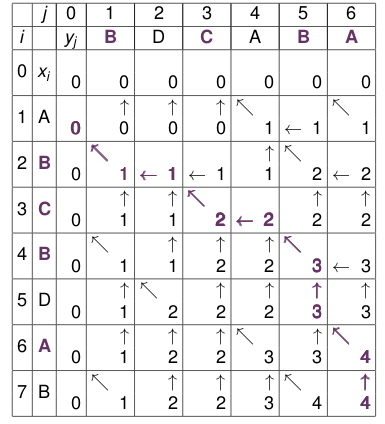
\includegraphics[scale=0.7]{algorithm}
\end{center}
\newpage
\section{Constructing an LCS}
\begin{lstlisting}[caption=PRINT-LCS({b,X,i,j})]
if i==0 or j==0 then
	return
if b[i,j] == "$\nwarrow$" then
	PRINT-LCS(b,X,i-1,j-1)
	print $x_i$
else if b[i,j] == "$\uparrow$" then
	PRINT-LCS(b,X,i-1,j)
else
	PRINT-LCS(b,X,i,j-1)
\end{lstlisting}
Initial call: PRINT-LCS(b,X,m,n)


\end{document}